\subsection{MDL Precision Error}
\label{ssc:mdl-error}

% In our experiments with linear manifold clusters, we use following definition of
% the minimum description length,
% \begin{equation} \label{eq:mdl-lmc-final}
% L(\varepsilon)
%     % = P_m [N + M(N - (M+1))/2 ]+ n(P_d\cdot M  + S(\varepsilon))
%     = P \sum^K_{k=1} \left[ N \cdot (N+3)/2 + 2 \sum^N_{m=M_k} Q_{mk}(\varepsilon) \right]
% \end{equation}
% where
% \begin{itemize}
% \item $N$ is the dimension of the space,
% \item $M$ is the dimension of the manifold,
% \item $n$ is a number of points in the linear manifold cluster,
% \item $P_m$ is the number of bits used for encoding each component of
% the manifold translation and the numbers required to calculate the basis vectors,
% \item $P_d$ is the number of bits used for encoding $M$ components of
% cluster point, projected on the linear manifold,
% \item $S(\varepsilon)$ is an entropy of a distribution of cluster points,
% in the orthogonal compliment subspace to the linear manifold of the cluster,
% calculated to be correct within an error bound of  $\varepsilon$,
% \item $\varepsilon$ is the specified quantization error.
% \end{itemize}

We are going to investigate the precision of the MDL calculations, in particular,
how changes in the encoding of the model and data affects resulting MDL value.

% Setup



For our experiments we used results of the climate clustering dataset,
see Section \ref{ssc:climate}. The climate dataset is the 24D dataset composed
of temperature and precipitation monthly averages for the period form 1951-1980.
We used cluster number 2, see Fig.~\ref{fig:cl-lmclus-c2}, which is a one
dimensional cluster, from the above clustering results.

\begin{figure}[H]
\centering
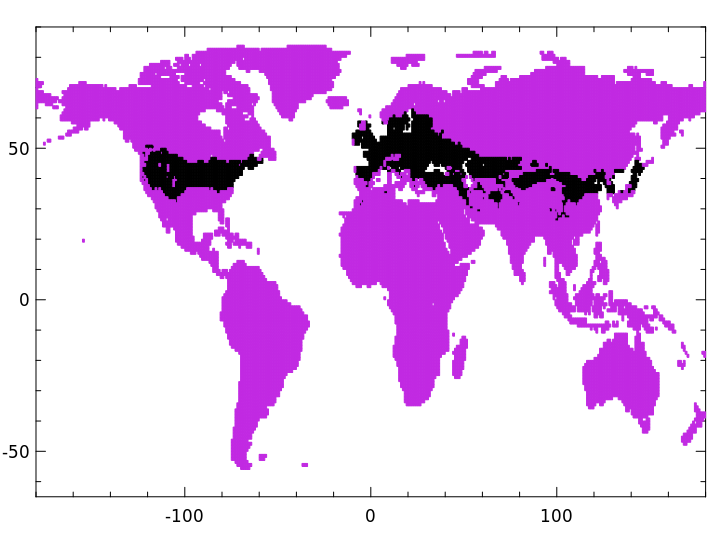
\includegraphics[width=3.5in]{img/CL02.png}
\caption{Cluster \#2 of the climate dataset created by LMCLUS algorithm, see Figure \ref{fig:cl-lmclus} in Section \ref{ssc:climate}.}
\label{fig:cl-lmclus-c2}
\end{figure}

First, we looked at the error introduced by the encoding of the data with
the lower precision then computations were done with. By default, $P_d$ constant
is set to 16 bits, which corresponds to the half-precision floating-point format,
\emph{Float16}. However, computations are usually done can be done in
the single-precision, \emph{Float32}, or double-precision floating-point format,
\emph{Float64}.

Error is calculated as difference between projected points in different
precision,
\begin{equation}
E_p = \frac{1}{n} \sum^n_{i=1} || B'x_i - q(B'x_i) ||^2
\end{equation}
where $B$ is the basis of the manifold in computational precision,
$x_n$ is the manifold point in computational precision,
$q$ is the conversion function from computational to encoding precision.

% precision error for projected data

\begin{juliaterm}
julia> #
# Encoding of the data from Float32 to Float16
prec_error(B,Xt,Float32,Float16)
1.5530144f-5

julia> 
# Encoding of the data from Float64 to Float16
prec_error(B,Xt,Float64,Float16)
1.5529915950350614e-5

julia> 
# Encoding of the data from Float64 to Float32
prec_error(B,Xt,Float64,Float32)
1.858106839030262e-9

\end{juliaterm}



Next, we verify that the quantization error within the user specified value
$\varepsilon$ for the encoding of the linear manifold cluster points in
the orthogonal compliment space. We calculated the average expected quantization
error $E$ and the average actual quantization error $E_q$.

% quantization error for projected data



\begin{table}[h]
\center
\begin{tabular}{ccc}
$\varepsilon^2$ & $E^2$ & $E_q^2$ \\
\hline
1.000e-04 & 1.005e-04 & 9.307e-03 \\
1.000e-06 & 9.994e-07 & 9.055e-05 \\
1.000e-08 & 1.000e-08 & 9.090e-07 \\
1.000e-10 & 1.000e-10 & 9.066e-09 \\



\end{tabular}
\caption{Average expected, $E$, and actual, $E_q$, quantization errors for
particular user-defined quantization error upper boundary $\varepsilon$.}
\label{tbl:quant-error}
\end{table}

Comparison results, see Table~\ref{tbl:quant-error} show that squared expected
quantization error \eqref{eq:sq-quant-error}, $E^2$, is under the user-defined
error upper boundary, $\varepsilon^2$. However, the actual squared quantization
error, $E_q$, resulted from quantizing the cluster points under calculated
quantization parameters \eqref{eq:quant-intervals}, is much larger then
expected one for a loose error boundary. But this error approaching to
its expected value as quantization error boundary tightens.
